\documentclass{bio}
%\documentclass[oupdraft]{bio}
\usepackage[colorlinks=true, urlcolor=citecolor, linkcolor=citecolor, citecolor=citecolor]{hyperref}
\usepackage[utf8]{inputenc}
\usepackage[english]{babel}

% Add history information for the article if required
%\history{}


%% NOTES TO SELF:
% Cite using:
%    \citet{...}  in text
%    \citealp{...}   within parantheses
%
% Temporary notifications and reminders:
%DIF < \newcommand\CHECK[2]{{\color{blue}#1}\NOTE{#2}}
%DIF -------
\usepackage{color} %DIF > 
%DIF < \newcommand\NB[1]{{\color{red}#1}}
\definecolor{NBcol}{rgb}{0.7,0,1} %DIF > 
%DIF < \newcommand\NOTE[1]{{\color{red}[#1]}}
\definecolor{CITEcol}{rgb}{1,0,0.7} %DIF > 
%DIF < \newcommand\CITE[1]{{\color{magenta}[#1]}}
\definecolor{COMMENTcol}{rgb}{0.7,0.2,0} %DIF > 
\newcommand\COMMENT[2]{\textcolor{COMMENTcol}{#1}\NOTE{#2}} %DIF > 
\newcommand\NB[1]{\textcolor{NBcol}{\textit{#1}}} %DIF > 
\newcommand\NOTE[1]{\NB{[#1]}} %DIF > 
\newcommand\CITE[1]{\textcolor{CITEcol}{[#1]}} %DIF > 
%DIF PREAMBLE EXTENSION ADDED BY LATEXDIFF
%DIF UNDERLINE PREAMBLE %DIF PREAMBLE
\RequirePackage[normalem]{ulem} %DIF PREAMBLE
\RequirePackage{color}\definecolor{RED}{rgb}{1,0,0}\definecolor{BLUE}{rgb}{0,0,1} %DIF PREAMBLE
\providecommand{\DIFaddtex}[1]{{\protect\color{blue}\uwave{#1}}} %DIF PREAMBLE
\providecommand{\DIFdeltex}[1]{{\protect\color{red}\sout{#1}}}                      %DIF PREAMBLE
%DIF SAFE PREAMBLE %DIF PREAMBLE
\providecommand{\DIFaddbegin}{} %DIF PREAMBLE
\providecommand{\DIFaddend}{} %DIF PREAMBLE
\providecommand{\DIFdelbegin}{} %DIF PREAMBLE
\providecommand{\DIFdelend}{} %DIF PREAMBLE
%DIF FLOATSAFE PREAMBLE %DIF PREAMBLE
\providecommand{\DIFaddFL}[1]{\DIFadd{#1}} %DIF PREAMBLE
\providecommand{\DIFdelFL}[1]{\DIFdel{#1}} %DIF PREAMBLE
\providecommand{\DIFaddbeginFL}{} %DIF PREAMBLE
\providecommand{\DIFaddendFL}{} %DIF PREAMBLE
\providecommand{\DIFdelbeginFL}{} %DIF PREAMBLE
\providecommand{\DIFdelendFL}{} %DIF PREAMBLE
%DIF END PREAMBLE EXTENSION ADDED BY LATEXDIFF
%DIF PREAMBLE EXTENSION ADDED BY LATEXDIFF
%DIF HYPERREF PREAMBLE %DIF PREAMBLE
\providecommand{\DIFadd}[1]{\texorpdfstring{\DIFaddtex{#1}}{#1}} %DIF PREAMBLE
\providecommand{\DIFdel}[1]{\texorpdfstring{\DIFdeltex{#1}}{}} %DIF PREAMBLE
%DIF END PREAMBLE EXTENSION ADDED BY LATEXDIFF

\begin{document}

\footnotetext{\color{blue}Manuscript version \DIFdelbegin \DIFdel{22 April 2014}\DIFdelend \DIFaddbegin \today\DIFaddend }

% Title of paper
\title{Methods that remove batch effects while retaining group differences may lead
to exaggerated confidence in downstream analyses
}

% List of authors, with corresponding author marked by asterisk
\author{VEGARD NYGAARD, EINAR ANDREAS RØDLAND, EIVIND HOVIG$^\ast$\\[4pt]
% Author addresses
\textit{Department of Tumor Biology,
Institute for Cancer Research,
Oslo University Hospital HF - Radiumhospitalet,
Montebello,
0310 Oslo,
Norway}
\\[2pt]
% E-mail address for correspondence
{ehovig@radium.uio.no}}

% Running headers of paper:
\markboth%
% First field is the short list of authors
{V. Nygaard, E. A. Rødland, E. Hovig}
% Second field is the short title of the paper
{Exagerated effects after batch correction}


\maketitle

% Add a footnote for the corresponding author if one has been
% identified in the author list
\footnotetext{To whom correspondence should be addressed.}

\begin{abstract}
{Removal of, or adjustment for, batch effects or centre differences is generally required when such effects are present in data. In particular, when preparing microarray gene expression data from multiple cohorts, array platforms, or batches for later analyses, batch effects can have confounding effects. Many methods and tools exist for this purpose. One method, ComBat which is part of the R package sva, is particularly popular due to its ability to remove batch differences even when batches are small and heterogeneous. It also has the option, recommended by the authors \NOTE{Anbefalt av dem alle eller kun av Johnson?}, of preserving the difference between study groups, estimated from a two-way ANOVA model, to avoid conflating batch effects and group differences during batch adjustments. Unfortunately, this recommended and frequently used approach may systematically induce incorrect group differences in downstream analyses when groups are distributed between the batches in an unbalanced manner. The scientific community seems to be largely unaware of this problem, which most likely has contributed to false discoveries being presented in the published literature.
}
\end{abstract}


\section{Introduction}\label{intro}

Extraneous variables, if left unaccounted for, have the potential to lead an investigator into drawing wrong conclusions. In molecular biology, extraneous variables are often called "batch effects", probably due to the fact that reagents and other equipment, for instance microarray chips, are made in batches, and this is frequently observed as an effect in the measurements. See \citet{Luo2010} for more examples. 

For a typical experiment comparing group differences, the presence of batch effects will decrease the statistical power since it adds variation to the data. If the batch--group design is unbalanced, i.e if the study groups are not equally represented in all batches, batch effects may act as a confounder and induce false differences between groups (\citealp{Leek2010}).

The standard way to handle an extraneous variable is to include it in the statistical model employed in the inquiry. However, many analysis tools for high throughput data do not cater for this option, and when available it could still be outside the competence of the investigator. Therefore, an alternative two step procedure has emerged. First the batch effects are estimated and removed, creating a ``batch effect free'' data set. In the next step, the statistical analyses are performed on the adjusted data without further consideration of batch effects. This appealing compartmentalization is also convenient for practical purposes, for example when data-processing and statistical analyses are performed by different personnel. \DIFaddbegin \DIFadd{Unfortunately, as we demonstrate in this paper, when the batch--group design is unbalanced, this approach may be unreliable.
}\DIFaddend 

\DIFdelbegin \DIFdel{The first step }\DIFdelend \DIFaddbegin \DIFadd{A simple removal of batch effects }\DIFaddend can be achieved by subtracting the mean of the measurements in one batch from all measurements in that batch, i.e mean adjustment or one-way ANOVA adjustment as implemented in the method \texttt{pamr.batchadjust} from the \texttt{pamr} package in R. When the batch--group design is balanced, mean-adjustment will remove most, but not necessarily all, variance attributed to batch and leave the between group variance, thus increasing the statistical power. However, when the batch--group design is unbalanced, batch differences will in part be \DIFdelbegin \DIFdel{influences }\DIFdelend \DIFaddbegin \DIFadd{influenced }\DIFaddend by group differences, and thus batch correction will reduce group differences and thereby reduce the statistical power. In very uneven group--batch designs with multiple groups, spurious group differences may even be induced in this way. Figure~\ref{fig:boxplots} illustrates both these effects.

To mitigate the above problems, one may simultaneously estimate batch effects and group differences, e.g. using a two-way ANOVA, and only remove the batch differences from the data. Effectively, \DIFdelbegin \DIFdel{this means }\DIFdelend group differences are estimated based on within batch \DIFdelbegin \DIFdel{comparison}\DIFdelend \DIFaddbegin \DIFadd{comparisons}\DIFaddend , and applied to the batch adjusted data. In a balanced group--batch design, group differences and batch effects are independent, and this approach becomes identical to the above described zero-centering per batch. If the group--batch design is heavily unbalanced, estimation of group differences and batch effects are interdependent. \DIFdelbegin \DIFdel{Unfortunately, when group differences estimated from an unbalanced group--batch design are applied to }\DIFdelend \DIFaddbegin \DIFadd{However, in applying the estimated group differences across }\DIFaddend the entire data set, \DIFdelbegin \DIFdel{if this batch adjusted data set is later analysed for group differences, the confidence will be exaggerated as the estimation of the group differences in the unbalanced design is less accurate than in the corresponding balanced design}\DIFdelend \DIFaddbegin \DIFadd{the uncertainties of these estimates are ignored. If the group--batch design is unbalanced and batch compositions ignored after batch adjustments have been made, later analyses will systematically underestimate the statistical uncertainties and exaggerate the confidence of group differences}\DIFaddend . Figure~\ref{fig:boxplots} illustrates how statistical uncertainties are deflated by this batch adjustment method by comparing them to the uncertainties from the original ANOVA.

The ComBat method described in \citet{Johnson2007}, and included in the sva package (\citealp{Leek2012}), can use either of the two above described approaches to estimate batch differences, but uses an empirical Bayes approach to avoid over-correction for batch effects for small batches. It has \DIFaddbegin \DIFadd{thus improved and }\DIFaddend popularised the two-way ANOVA procedure for retaining group differences when adjusting for batch effects, and the inclusion of group difference as a covariate when removing batch effects has been recommended \CITE{reference}. Based on actual use of ComBat by the authors and others, we suspect thus adjusted data are commonly treated as      \DIFdelbegin \DIFdel{"}\DIFdelend \DIFaddbegin \DIFadd{``}\DIFaddend batch effect free\DIFdelbegin \DIFdel{" }\DIFdelend \DIFaddbegin \DIFadd{'' }\DIFaddend in subsequent analysis. And as a consequence, confidence in group effects has been overestimated and false results reported.

\DIFdelbegin %DIFDELCMD < \NB{Kort oppsummere behovet for batch-korrigering: generelt og i microarraydata.}
%DIFDELCMD < %%%
\DIFdelend \DIFaddbegin \DIFadd{Statisticians would most likely take extra precautions should the sample or batch sizes be very small. However, the effects of batch adjustment using two-way ANOVA or ComBat on unbalanced data sets remain even as sample and batch sizes increase. For example, group comparisons using one-way ANOVA on the batch adjusted data will essentially result in $F$ statistics that are inflated by a fixed factor which depends on the unevenness of the design rather than the size of the sample or batches. The effect of this may be further exacerbated by running these analyses a large number of times, e.g. on thousands of genes, and use false discovery rate to determine significant cases: an approach that is particularly sensitive to inflated false positive rates.
}\DIFaddend 


\DIFdelbegin %DIFDELCMD < \NB{Kort beskrive metoder som gjoer dette (batch-sentrering, ANOVA, ComBat).}
%DIFDELCMD < 

%DIFDELCMD < \NB{Forklare tilsiktet effekt disse paa batch+gruppe-forskjeller (balansert versus ikke-balansert).}
%DIFDELCMD < 

%DIFDELCMD < \NB{Forklare kort hva faktisk effekt er: ANOVA gir redusert gruppe-forskjeller, mens for ComBat overestimeres den statistiske styrken/sikkerheten av forskjellen.}
%DIFDELCMD < 

%DIFDELCMD < %%%
\DIFdelend \section{Methods for batch effect correction}

\subsection{Model for data with batch effects}

We will base our discussion \DIFdelbegin \DIFdel{of data with batch effects }\DIFdelend on a simple model \DIFaddbegin \DIFadd{for data with batch effects}\DIFaddend :
\begin{equation}
Y_{ijr}=\alpha+\beta_j+\gamma_i+\epsilon_{ijr}
\end{equation}
where $i=1,\ldots,m$ are the different batches, $j=1,\ldots,M$ are different study groups that we wish to compare, and $r=1,\ldots,n_{ij}$ are the different samples within batch $i$ and group $j$.

When combining data from more diverse data sources, e.g. microarray data from different platforms, a more general model is required. One such model, used by \citet{Johnson2007}, is
\begin{equation}
Y_{ijgr}=\alpha_g+X_r\beta_{g}+\gamma_{ig}+\delta_{ig}\epsilon_{ijgr}
\end{equation}
where $g=1,\ldots,G$ are different measurements, e.g. genes, performed for each sample, and $X$ is the design matrix which in our case will indicate the study group. This permits independent rescaling of data from different batches. In addition, \citet{Johnson2007} uses an empirical Bayes approach to estimate $\gamma_{ig}$ and $\delta_{ig}$ to stabilise estimates, which is critical for use with small batches.

For simplicity, we consider the case with a single gene and constant scale, i.e. $\delta_{ig}=1$. We will discuss the effect of empirical Bayes estimation of $\gamma_{ig}$ later, but \DIFdelbegin \DIFdel{out }\DIFdelend \DIFaddbegin \DIFadd{our }\DIFaddend main argument is more easily made in the simpler context. \DIFaddbegin \DIFadd{Empirical Bayes may reduce the amount of batch adjustment in cases where batch effects are small or cannot be accurately estimated, e.g. for small batches. However, in cases with large batches or substantial batch effects, it should differ little from the two-way ANOVA approach.
}\DIFaddend 

\subsection{Standard batch correction methods}

\DIFdelbegin \DIFdel{The main }\DIFdelend \DIFaddbegin \DIFadd{A common }\DIFaddend ambition of batch effect adjustments is to \DIFdelbegin \DIFdel{be able to }\DIFdelend remove batch differences in such a way that downstream analyses of the adjusted data may be done without further \DIFdelbegin \DIFdel{batch adjustments}\DIFdelend \DIFaddbegin \DIFadd{corrections for batches}\DIFaddend .

The most common method for removing batch effects is to zero-centre each batch:
\begin{equation}
\Delta\widetilde Y_{ijr}=Y_{ijr}-\bar{Y}_{i}
\quad\text{where}\quad
\bar{Y}_i=\frac{\sum_{j=1}^M\sum_{r=1}^{n_{ij}} Y_{ijr}}{\sum_{j=1}^M n_{ij}}.
\end{equation}
An alternative is to centre each batch to the common average by adding the average value $\bar{Y}$ across the entire data set: i.e. $\widetilde Y_{ijr}=\Delta\widetilde Y_{ijr}+\bar{Y}$. When comparing groups, the common value $\bar{Y}$ has no effect, and so this is equilvalent to zero-centring each batch. \DIFdelbegin \DIFdel{However, if the different }\DIFdelend \DIFaddbegin \DIFadd{If the }\DIFaddend groups are unevenly represented in the different batches, the batch average $\bar{Y}_i$ will tend to capture group differences as well as batch effects\DIFdelbegin \DIFdel{. }\DIFdelend \DIFaddbegin \DIFadd{:
}\begin{equation}
\DIFadd{\Delta}\widetilde{Y}\DIFadd{_{ijr}=\beta_j-}\bar{\beta}\DIFadd{_i+\epsilon_{ijr}-}\bar{\epsilon}\DIFadd{_i
}\quad\DIFadd{\text{where}}\quad
\bar{\beta}\DIFadd{_i=\frac{\sum_{j=1}^M n_{ij}\beta_j}{\sum_{j=1}^M n_{ij}},}\;
\bar{\epsilon}\DIFadd{_i=\frac{\sum_{j=1}^M\sum_{r=1}^{n_{ij}} \epsilon_{ijr}}{\sum_{j=1}^M n_{ij}}.
}\end{equation}
\DIFaddend Thus, batch centering \DIFdelbegin \DIFdel{may }\DIFdelend \DIFaddbegin \DIFadd{will tend to }\DIFaddend reduce group differences \DIFaddbegin \DIFadd{in an unbalanced design}\DIFaddend , and thus reduce the power of downstream analyses. \DIFaddbegin \DIFadd{By reducing the differences between some groups, i.e. those found together in the same batches, it may also induce false differences between other groups.
}\DIFaddend 

Removing batch effects while retaining group differences can be done through \DIFdelbegin \DIFdel{an ANOVA analysis in which the }\DIFdelend \DIFaddbegin \DIFadd{a two-way ANOVA in which }\DIFaddend group effects, $\beta_j$, and \DIFdelbegin \DIFdel{the }\DIFdelend batch effects, $\gamma_i$, are estimated simultaneously. Batch adjusted values may then be obtained by subtracting the estimated batch effects, \DIFdelbegin \DIFdel{$\hat\beta_j$}\DIFdelend \DIFaddbegin \DIFadd{$\hat\gamma_i$}\DIFaddend :
\begin{equation}
\widetilde Y_{ijr}=Y_{ijr}-\hat\beta_j=\alpha+\DIFdelbegin \DIFdel{(\beta_j}\DIFdelend \DIFaddbegin \DIFadd{\beta_j+(\gamma_i}\DIFaddend -\hat\DIFdelbegin \DIFdel{\beta_j)+\gamma_i}\DIFdelend \DIFaddbegin \DIFadd{\gamma_i)}\DIFaddend +\epsilon_{ijr}.
\end{equation}
This will yield batch adjusted values where any systematic bias induced by the batch differences has been removed, while the group differences are retained.

\DIFdelbegin \DIFdel{Unfortunately, the estimation error $\hat\beta_j-\beta_j$ }\DIFdelend \DIFaddbegin \DIFadd{The estimation error $\hat\gamma_i-\gamma_i$ }\DIFaddend affects all values within the same batch in the same manner\DIFdelbegin \DIFdel{, inducing a dependency between the values. If the study groups are evenly represented in all batches, this will not influence estimated group differences as all groups are equally affected. However, if groups are unevenly represented, this induced dependency can have severe impact on downstream analyses. }\DIFdelend \DIFaddbegin \DIFadd{. Thus, while the aim is to remove spurious dependencies within batches, it may also induce new dependencies. In a balanced group--batch design, this has the same effect on all groups and thus does not influence group comparisons. In an unbalanced design, however, the estimated batch effects $\hat\gamma_i$ will correlate with the estimated group effects $\hat\beta_j$. }\COMMENT{Assuming the batch adjusted values are without further batch differences corresponds to assuming that $\gamma_i=\hat\gamma_i$, and ignoring the estimation uncertainty and its impact on the correlated $\hat\beta_j$. It results in over-confidence in the accuracy of the group differences, which can have severe impact on downstream analyses.}{Denne forklaringen må jeg gjøre mye klarere.}
\DIFaddend 


\section{Results}

\subsection{A simple sanity check}

The undesired consequences of preserving group effects when correcting for batch effect is readily illustrated with a sanity check using random numbers . The documentation accompanying the sva library has a runnable example demonstrating how to adjust a data set with ComBat followed by a F-test. Swapping the real data with random numbers from a normal distribution (mean=0, sd=1), but otherwise following the instructions, will generate the p-value distribution shown in Figure\DIFdelbegin \DIFdel{1. }\DIFdelend \DIFaddbegin \DIFadd{~\ref{fig:p-sva}. }\NOTE{Perhaps show Q-Q plot of $F$-statistics.} \DIFaddend The skewed distribution is a indication that this approach may have a unintentional adverse effect. \DIFdelbegin %DIFDELCMD < \NOTE{Jeg har ikke beskrevet permutatsjon checken fordi jeg er usikker paa om vi skal bruke den.}
%DIFDELCMD < %%%
\DIFdelend \DIFaddbegin \NOTE{Tror vi dropper permutasjonstesten.}
\DIFaddend 

%DIF < % FIGURE 1: Original position
\DIFaddbegin \DIFadd{If the number of samples is increased, the empirical Bayes estimates used by ComBat will shrink the batch effect estimates and thus moderate the batch adjustments. However, if random data with different means in each batch, but no difference betwene groups, are drawn, the problem remains. }\NOTE{Bør dette komme her eller senere? Evt. understøttes?}
\DIFaddend 

%DIF > % FIGURE 1=fig:p-sva: Original position
\DIFaddbegin 

\DIFaddend \subsection{Explanation for the simple two-group comparison}

To explain more clearly what is happening, and quantify the size of the problem, we may consider the simple case of estimating the difference $\Delta\beta=\beta_A-\beta_B$ between two groups, $A$ and $B$, when there are $m$ batches with batch $i$ containing $n_{iA}$ and $n_{iB}$ samples from each of the two groups for $i=1,\ldots,m$.

If we estimate the group difference within batch $i$, we get
\begin{equation}
\widehat{\Delta\beta}_i=\bar{Y}_{iA}-\bar{Y}_{iB}\sim\text{N}\left(\Delta\beta,\frac{\sigma^2}{\nu_i}\right)
\quad\text{where}\quad
\bar{Y}_{ij}=\frac{\sum_{r=1}^{n_{ij}}Y_{ijr}}{n_{ij}},\,
\nu_i=\frac{1}{\frac{1}{n_{iA}}+\frac{1}{n_{iB}}},
\end{equation}
from which we may express the overall estimate of $\Delta\beta$
\begin{equation}
\widehat{\Delta\beta}=\frac{\sum_{i=1}^m \nu_i\,\widehat{\Delta\beta}_i}{\nu}
\sim\text{N}\left(\Delta\beta,\frac{\sigma^2}{\nu}\right)
\quad\text{where}\quad
\nu=\sum_{i=1}^m\nu_i.
\end{equation}

If batch and group effects are estimated using a two-way ANOVA, the estimate $\widehat{\Delta\beta}$ will be as stated above, and so the estimated group difference is unaffected. The batch effects are then removed, and the estimated group differences retained, leaving the estimated $\widehat{\Delta\beta}$ unchanged by the batch adjustment. However, if this batch adjusted data set is analysed without considering batch effects, the variance of $\widehat{\Delta\beta}$ will be computed under the assumption that it is derived from a comparison of $n_A=\sum_{i=1}^m n_{iA}$ versus $n_B=\sum_{i=1}^m n_{iB}$ samples, and thus satisfy
\begin{equation}
\widehat{\Delta\beta}
\sim\text{N}\left(\Delta\beta,\sigma^2\cdot\left(\frac{1}{n_A}+\frac{1}{n_B}\right)\right).
\end{equation}
Using Jensen's inequality, we may then derive
\begin{equation}
\frac{1}{\frac{1}{n_A}+\frac{1}{n_B}}=n\cdot\frac{n_A}{n}\cdot\frac{n_B}{n}
\le
\nu
=\sum_{i=1}^m \frac{1}{\frac{1}{n_{iA}}+\frac{1}{n_{iB}}}
=\sum_{i=1}^m n_i\cdot\frac{n_{iA}}{n_i}\cdot\frac{n_{iB}}{n_i}
\end{equation}
with equality if and only if the ratios $n_{iA}:n_{iB}=n_A:n_B$ for all batches $i=1,\ldots,m$.



\subsection{Examples of undesired consequences}

As the amount of false positive results when trying to retain group differences depends on the batch/group balance, we will show two examples with varying degree of unbalancedness. 

\DIFdelbegin \DIFdel{1) }\DIFdelend \DIFaddbegin \subsubsection{\DIFadd{Experiment 1}}

\DIFaddend In the first experiment(\citealp{Towfic2014}), cells were treated with glatiramer acetate (a medicine for multiple sclerosis) or a generic and mRNA was measured using microarrays alongside control samples. A batch effect correlating to the chip (Illumina WG-6\_V2, six samples per chip) was observed and adjusted for with ComBat, whereafter the data was tested for differetially expressed genes, yielding a list of 1000 genes (Table S5, \citealp{Towfic2014}). Unfortunately the batch/treatment design was unbalanced with several batches having only one of the main treatments of interest. When we re-analyzed their data without using ComBat, but instead blocked for batch effect in limma, only 9 genes were found ($\text{FDR}<0.05$). \DIFaddbegin \NOTE{Also run analysis using a mixed random effects model which assumes random batch effects much like in the empirical Bayes model.} \DIFaddend Additional sanity checks with random numbers or perumted labels were also carried out and the distribution of p-values for differents settings are shown in \DIFdelbegin \DIFdel{Fig.  2.  }\DIFdelend \DIFaddbegin \DIFadd{Figure~\ref{fig:p-towfic}.  }\DIFaddend Our conclusion is that most of the genes reported as differtially expresssed in (\citealp{Towfic2014}) are false positives. This example is a sort of "worst case" scenario for applying ComBat, since it both has a very unbalanced batch/group design and a a priori assumpotion of no difference. The R-code for our analysis and a more extensive report can be downloaded from github (\href{https://github.com/vegardny/combat_tests.git}).

%DIF < % FIGURE 2: Original position
%DIF > % FIGURE 2=fig:p-towfic: Original position

\DIFdelbegin \DIFdel{2) }\DIFdelend \DIFaddbegin \subsubsection{\DIFadd{Experiment 2}}

\DIFaddend The second example is taken from the supporting information for the original ComBat article (\citealp{Johnson2007}) where it is denoted "data set 2". Cells inhibited for the expression of the TAL1 gene were compared to controls on a microarray platform. The experiment was conducted on three different time points (used as batches) with a total of 30 samples and a fairly balanced batch/treatment set up (6-2, 3-4 and 9-6). ComBat was applied followed by a t-test in order to identify differentially expressed genes. First, we reproduced their analysis including the adjustment by ComBat, but using limma instead of the t-test, resulting in 1003 probes (q<0.05).  Then, we analysed their data without batch adjustment in ComBat, but blocking for batch in limma, resulting in 377 probes (q<0.05). In addition the two sanity checks outline above were performed. In contrast to the above results obtained for(\citealp{Towfic2014}), the P-value distributions for the alternative analyses (\DIFdelbegin \DIFdel{Fig.3 }\DIFdelend \DIFaddbegin \DIFadd{Figure~\ref{fig:p-johnson} }\DIFaddend a,b) does not indicate a huge difference. Nevertheless, we belive that  P-values are deflated for the ComBat adjusted analysis. The R-code for our analysis and a more extensive report can be downloaded from github (\href{https://github.com/vegardny/combat_tests.git}).

%DIF < % FIGURE 3: Original position
%DIF > % FIGURE 3=fig:p-johnson: Original position

%DIF < % FIGURE 4: Original position
%DIF > % FIGURE 4=fig:pdist-johnson: Original position

\DIFdelbegin \DIFdel{3) }\DIFdelend \DIFaddbegin \subsubsection{\DIFadd{More?}}

\DIFaddend \NOTE{Her kan vi fylle paa med flere eksempler etter samme mal hvis det trengs. Feks en fersk artikkel fra Nature Genetic (\citealp{Yoo2014}). Der har de kombinert sekvenseringsdata  (deres data) fra 9 lymfom pasienter med et (eksternt) microarray data set som har 6 lymfom proever og 5 kontroller, dvs kontroll gruppen er helt fravaerende hos dem. Dvs veldig ubalansert (9/0, 6/5), MEN skille mellom phenotypene er saa stor at de sikkert hadde funnet omtrent de samme genene signifikante med aa bare bruke de balanserte dataene (men det var jo ikke deres.) Dette er ikke en viktig del av paperet, men det er veldig feil selvom konsekvensense ikke blir store. Dog gir det et falskt inntrykk av at dataene deres ligner tidligere data, se heatmap i suppl.. Dessuten lager de GO analyser av dette som egentlig er 7 aar gamle andres data og ikke deres}


\section{Discussion}

\DIFaddbegin \NB{Systematic underestimation of $P$-values combined with FDR is a particularly bad combination as FDR lends strength across tests.}

\DIFaddend \subsection{Increased emphasis on preserving group difference}

In the original ComBat article (\citealp{Johnson2007}) it is clear that the primary motivation behind ComBat was to employ an Emprical Bayes method for batch-effect removal \DIFaddbegin \DIFadd{to allow better handling of small batches}\DIFaddend . The feature of retaining group differences for unbalanced designs is optional and seems to be subordinate, only exemplified in the supplementary information. However, over the years this feature became more important judging from advice given by the author to users
(
[1](\href{https://groups.google.com/d/msg/combat-user-forum/eSVSKwGtuyE/ZIWV2juYmmAJ})
,[2](\href{https://groups.google.com/d/msg/combat-user-forum/Vkb9p7wekd4/h5Etie7FTVQJ})
,[3](\href{https://groups.google.com/d/msg/combat-user-forum/fpBTcgDjiR8/uo4QIZL4sZgJ})
,[4](\href{https://groups.google.com/d/msg/combat-user-forum/26FZlgU2LFQ/W6U_Lhh_64EJ})
). \NOTE{Aa linke direkte er kanskje litt ufint, alternativt kan det linkes til forumet uten konkrete innlegg.}  
\DIFdelbegin \DIFdel{And when ComBat was }\DIFdelend \DIFaddbegin \DIFadd{When ComBat was later }\DIFaddend incorporated in the sva package (\citealp{Leek2012}), \DIFdelbegin \DIFdel{inclusion of group labels was made almost mandatory (an undocumented option of passing a NULL value exists)}\DIFdelend \DIFaddbegin \COMMENT{batch adjustment without covariates was no longer a default as specification of covariates became a requirement, although specification of a null model was still possible although not clearly documented in the sva documentation}{Is this correct?}\DIFaddend . Thus, \DIFdelbegin \DIFdel{this problematic use has likely been }\DIFdelend \DIFaddbegin \DIFadd{we expect this usage to have grown more }\DIFaddend common.


\subsection{Motivation for this warning}

Our knowledge of ComBat came through a typical use case when trying to salvage unbalanced data which had batch effects. Upon realizing that the confidence on our group differences were exaggerated, the literature was searched for a better understanding of correct use and potential overseen limitations of ComBat. But the authors of ComBat and the sva package recommended our usage (\citealp{Johnson2007}, \citealp{Leek2012}). In addition, other works looking into the problem of batch effects were mostly recommending ComBat without much concern (\citealp{Kupfer2012}, \citealp{Kitchen2011}). A brief inquiry into  some of the articles citing ComBat (574 Google Scholar) revealed few problems, and their method descriptions regarding ComBat were mostly sparse, limited to one or two sentences (\CITE{24391845}, \CITE{18414638}, \CITE{21731603}, \CITE{23630272}, \CITE{24584070}). A further indication of their carefree use of this potentially devastating procedure was the frequent neglect to state the program parameters, i.e batch labels (\CITE{18414638}, \CITE{21731603}) or group labels (\CITE{24391845}, \CITE{18414638}, \CITE{21731603}, \CITE{23630272}, \CITE{23482648}, \CITE{24584070}). Often no effort was done in order to substantiate the existence of batch effects in their data, except for stating the presence of batches (\CITE{24391845}?, \CITE{18414638}, \CITE{21731603}, \CITE{23630272}). In one instance ComBat was even applied on data were effects due to batch were investigated, but not found \NOTE{husker ikke ref}. The incorporation of the method into analysis pipelines (\CITE{16642009}, TCGA) and other packages (\CITE{23452776}, \CITE{21937664}) could make its usage even more trivial and parameters setting harder to perceive.
Taken together we fear that many published results from data adjusted by ComBat are completely or partially false. \DIFdelbegin \DIFdel{And knowing that scientists don't give up where one analysis fails, a method that almost ensures a result given a sufficiently unbalanced design will continue to be used.
}\DIFdelend \DIFaddbegin \COMMENT{And knowing that scientists don't give up where one analysis fails, a method that almost ensures a result given a sufficiently unbalanced design will continue to be used.}{Dette bør nok formuleres anderledes.} \NOTE{Her bør vi nok fokusere tydeligere på bruk der gruppe er brukt som kovariat. Om dette er uklart, bør vi sjekke det før vi lister det opp.}
\DIFaddend 


\subsection{Practical advice}

We have shown that adjusting for batch effects while preserve the group difference may lead to varying degree of false results. Knowing this, to what degree can an investigator trust a result from a work applying such a method? Essentially, when the batch/group configuration is balanced, or group difference is ignored  (i.e. no group labels not given as parameters to ComBat), problems related to preserving group differences will not occur. For other cases, a re-analysis without using this approach is the most rigorous path. However, this thoroughness is not feasible if the downstream  analysis can not adjust for batch effects by it self. To reach a reliable result, batch effects need to be handled in some way or another. To make matters worse, a re-analysis relies on the availability of the raw data and a description of processing and analysis steps taken in the original work. Even when this is available, the necessary bioinformatic skills and work hours could still be in short supply. For such situations, a superficial assessment can be performed, taking special note of batches were groups of interest are near missing and how likely a group difference is. In essence asking if the balanced parts (effective sample size?) of the data has enough power to detect the presumed effects and if this is the case (\citealp{Johnson2007}, \CITE{24584070}), treat the results more like an ordered list with the most likely true positives on top while de-emphasizing the somewhat deflated p-values . In contrast, if biological knowledge suggest that a group effect is unlikely  (\CITE{24391845}, \CITE{18414638}?, \CITE{21731603}, \CITE{23630272}), an intermediate lack of batch/group balance  could lead to a mostly false result.


\section{Supplementary Material}
\label{supp}

Supplementary material is available online at
\href{http://biostatistics.oxfordjournals.org}%
{http://biostatistics.oxfordjournals.org}.

\section*{Reproducible research}
\NOTE{vi boer klare aa tilfredstille kravene i http://biostatistics.oxfordjournals.org/content/10/3/405.full}


\section*{Acknowledgments}

[...Acknowledgements...]
{\it Conflict of Interest}: None declared.


\bibliographystyle{biorefs}
\bibliography{D:/Projects/_Appl_/_TeX_/library}
%\bibliography{refs}


%\begin{figure}[!p]
%\centering\includegraphics{fig1.eps}
%\caption{...}
%\label{Fig1}
%\end{figure}

\begin{figure}[!p]
\centering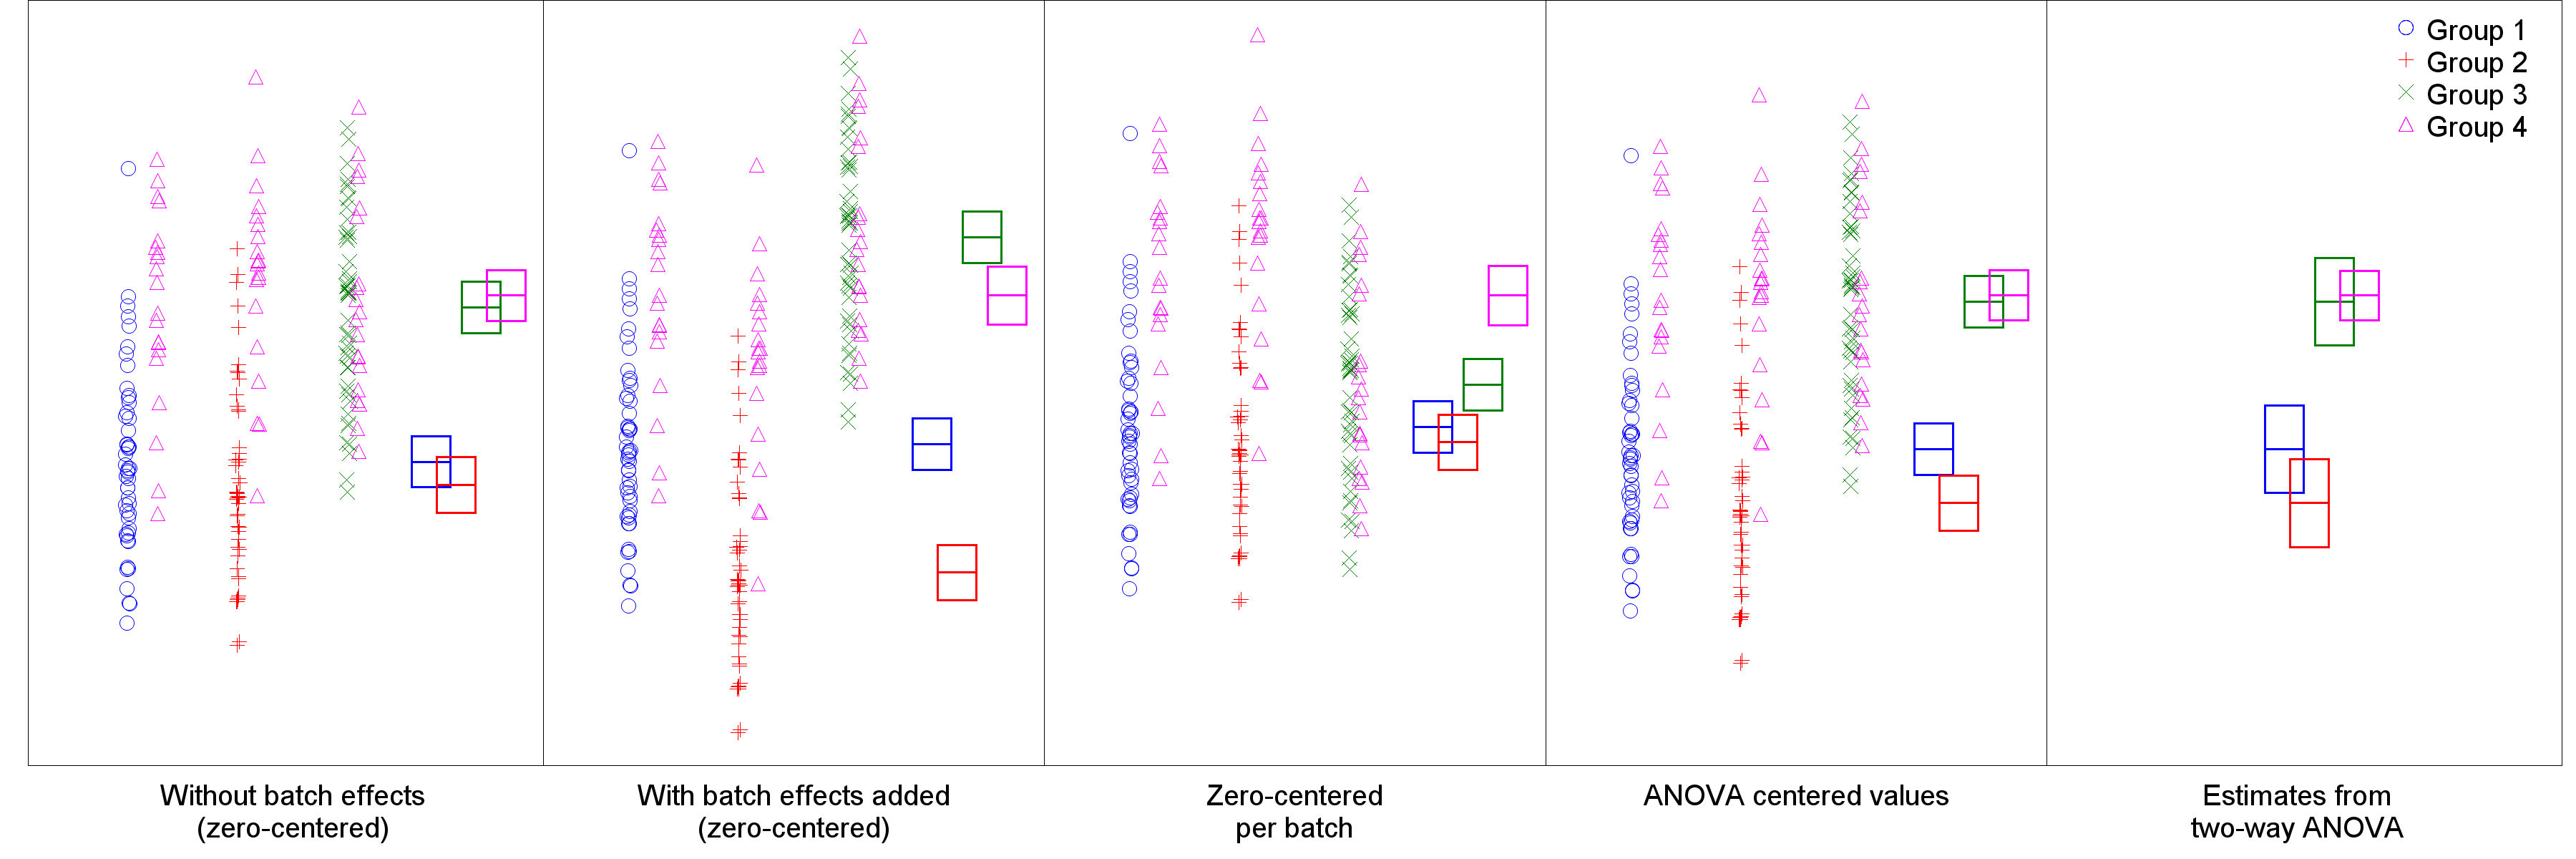
\includegraphics[width=13cm]{Fig/boxplots.png}
\caption{Simulated data from four study groups was generated where groups 1 and 2 have lower means than groups 3 and 4. These were placed in three different batches with batch effect added. Values and boxes showing mean and two standard errors of the mean are displayed for data without batch effects, after adding batch effects, after batch centering, and after ANOVA based batch centering. The last frame shows the least squares estimates of the group means from a two-way ANOVA analysis with 2 standard errors. This case, design and effects, was selected to illustrate the spurious effects that may arise.}
\label{fig:boxplots}
\end{figure}


\begin{figure}[!p]
\centering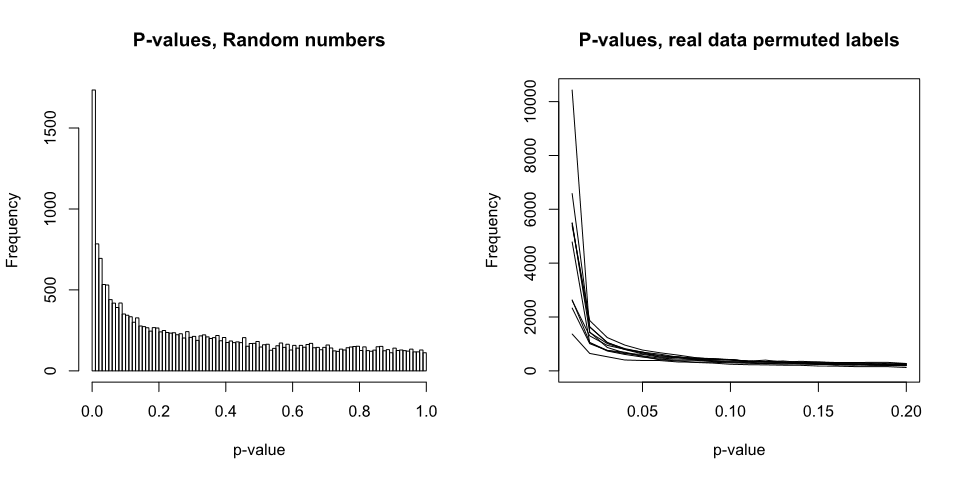
\includegraphics[width=13cm]{Fig/pvaluesleeksva.png}
\caption{
Two sanity checks were the recommended use of ComBat fails. Adapted from the user guide in the sva package. 
a) Real data is substituted with random numbers from a normal distribution (mean=0, sd=1), but the batch/group design is retained, followed by batch adjustment in ComBat and a F-test.
b) 10 runs of real data with the "cancer" labels permuted within batches, followed by ComBat adjustment and a F-test. All permutations produces a skewed p-value distribution.
}
\label{fig:p-sva}
\end{figure}

\begin{figure}[!p]
\centering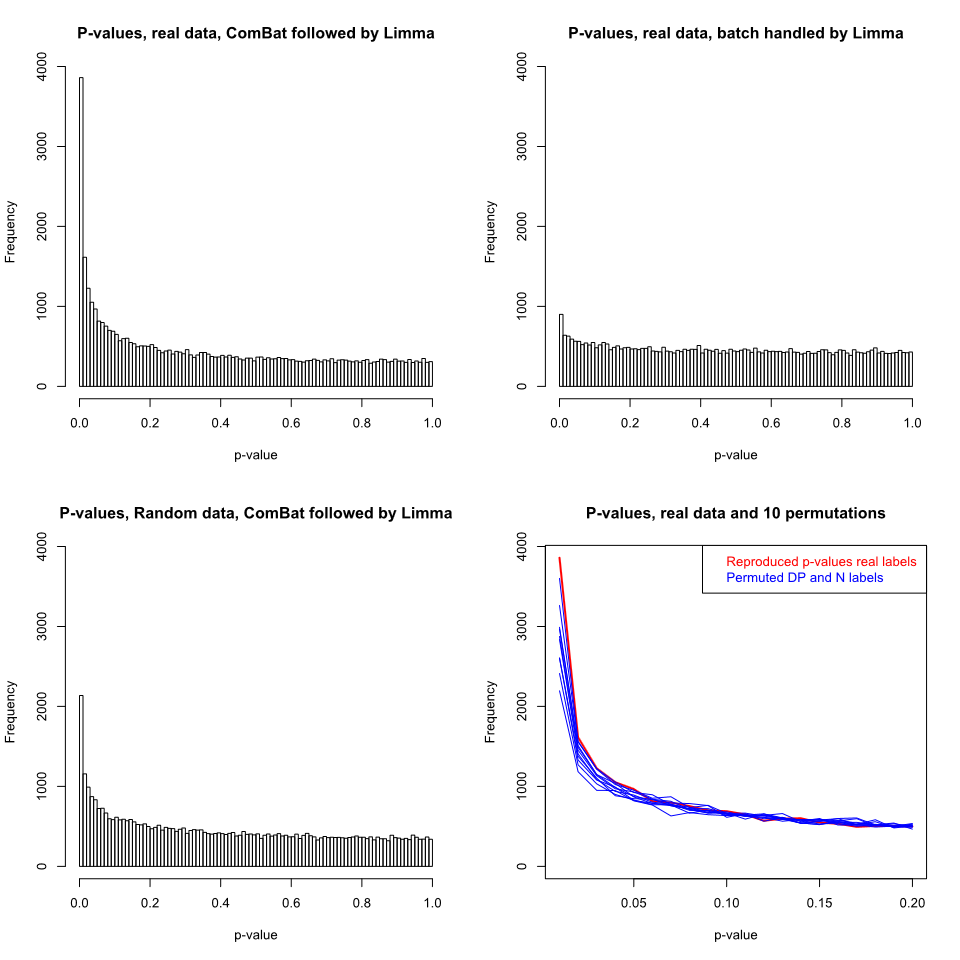
\includegraphics[width=13cm]{Fig/pvaluestowfic.png}
\caption{
P-value distribution for the main comparison in (data set 2 24421904) glatiramer acetate vs. generic.  
a) Real data adjusted by ComBat as described in the article followed by a significance test in limma. 
b) Real data not adjusted by ComBat, tested for significance in limma using batch as a blocking factor. 
c) Real data is substituted with random numbers from a normal distribution (mean=0, sd=1), but the batch/group design is retained, followed by batch adjustment in ComBat and a significance test in limma.
d) 10 runs of real data with the glatiramer acetate("DP") and generic("N") labels permuted within batches, followed by ComBat adjustment and significance test in limma.  
\NOTE{jeg tok med begge sanitycheckene her. Er d) slik einar foreslo?. Merk jeg har ikke permutert alle labeler, bare de mellom DP og N. Det er en del andre.}
}
\label{p-towfic}
\end{figure}

\begin{figure}[!p]
\centering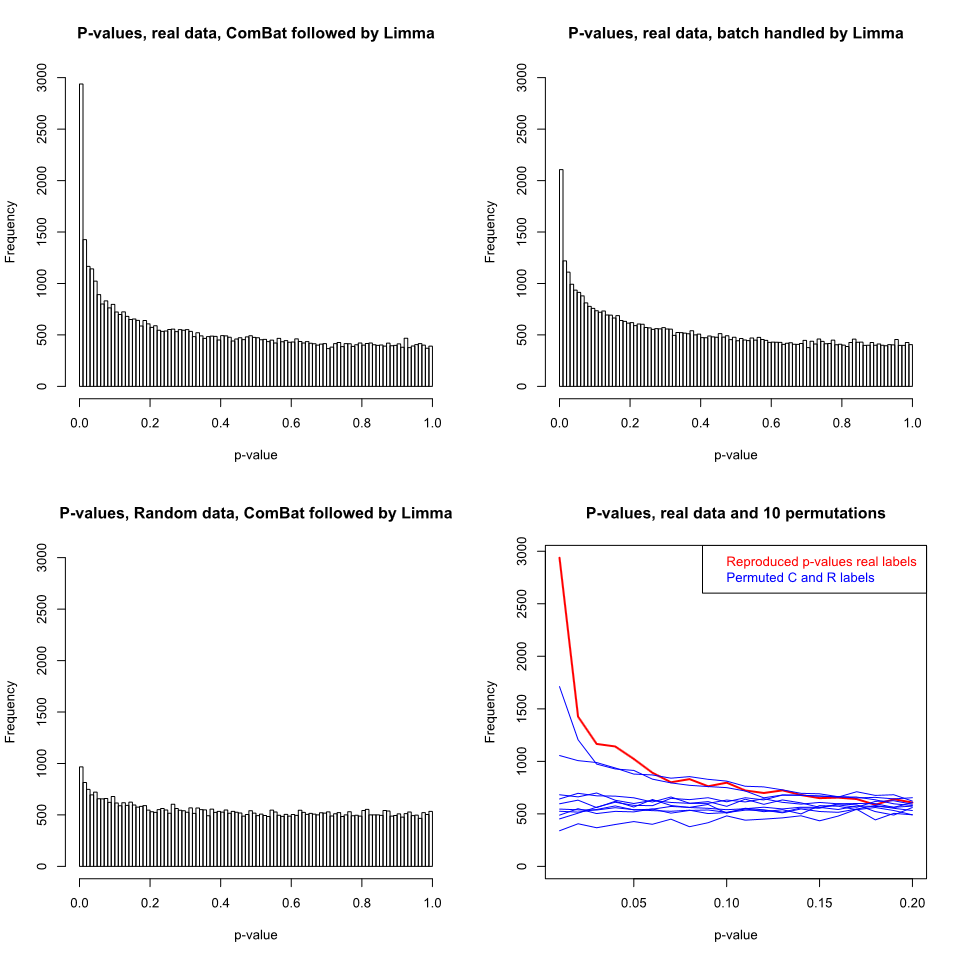
\includegraphics[width=13cm]{Fig/pvaluesjohnson.png}
\caption{
P-value distribution for the main comparison in (data set 2, \citealp{Johnson2007}) for  
a) Real data adjusted by ComBat as described in the article followed by a significance test in limma. 
b) Real data not adjusted by ComBat, tested for significance in limma using batch as a blocking factor. 
c) Real data is substituted with random numbers from a normal distribution (mean=0, sd=1), but the batch/group design is retained, followed by batch adjustment in ComBat and a significance test in limma.
d) 10 runs of real data with the group labels permuted within batches, followed by ComBat adjustment and significance test in limma.   
\NOTE{Problemet med permutatsjons sanitychechen slik jeg har utfoert og plottet den her er at den neppe kan sies aa feile. Dessuten kan de 3 foerst plottene bli plottet i ett som vist under i en alternativ version jeg synes er finere, men dette gaar ikke for permutasjonstesten tror jeg}
}
\label{fig:p-johnson}
\end{figure}

\begin{figure}[!p]
\centering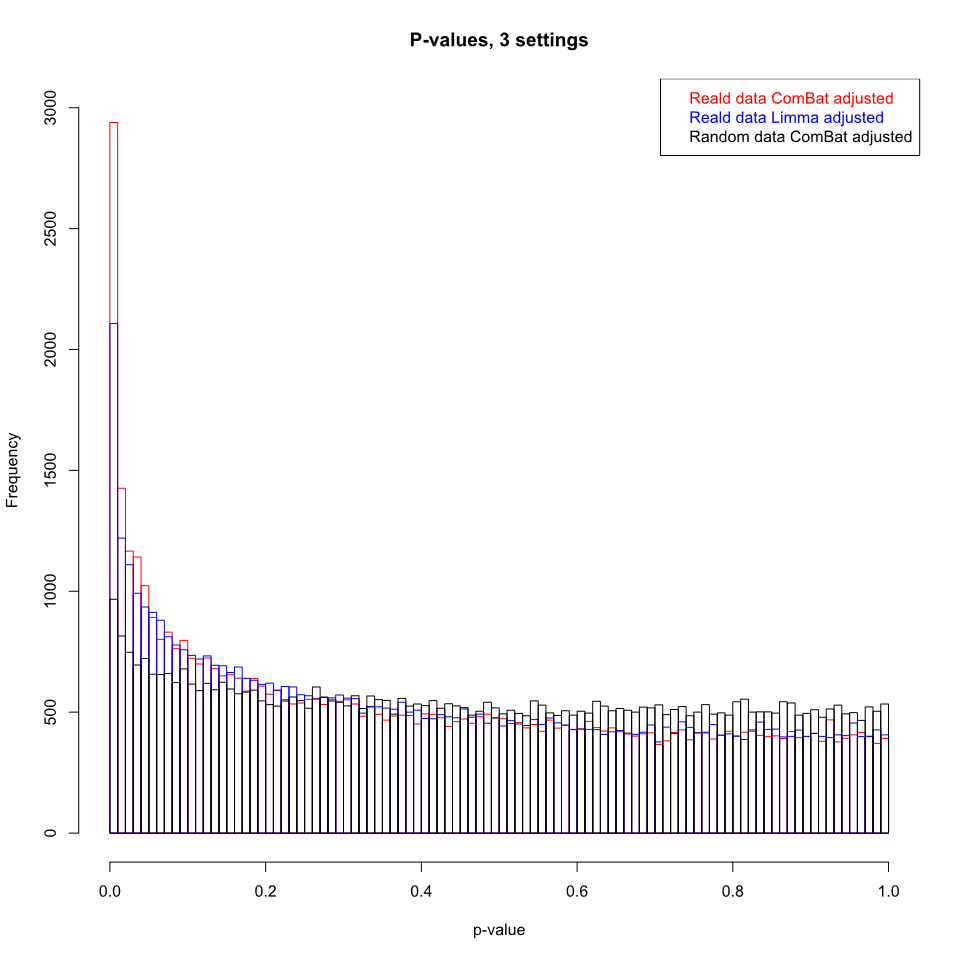
\includegraphics[width=13cm]{Fig/pvaluesjohnson2.png}
\caption{
\NOTE{Alternativ illustrasjon av de tre p-value distribusjonene}
}
\label{fig:pdist-johnson}
\end{figure}


%\begin{table}[!p]
%\tblcaption{... \protect\citet{...} ... \label{Table1}}
%{\tabcolsep=4.25pt
%\begin{tabular}{@{}cccccccccc@{}}
%\tblhead{Dis & Chr & Marker & MLE-OR & MLE & MLE & EB-HM-OR & EB-HM & EB-HM & ES \\
%&&& (SE) & \textit{P}-value & rank & (SE) & \textit{P}-value & rank & rank}
%CAD & 2 & rs2943634 & 1.22(0.04) & $1.23 \times 10^{-5}$ & 32 & 1.02(0.01) & 0.19 & 28 & 37 \lastline
%\end{tabular}}
%\end{table}

\end{document}

